\documentclass[10pt]{beamer}
%\documentclass[handout,10pt]{beamer}

\usetheme[progressbar=frametitle]{metropolis}

\usepackage{booktabs}
\usepackage[scale=2]{ccicons}


\usepackage{amsmath}
\usepackage{pgfplots}
\usepgfplotslibrary{dateplot}

\usepackage{xspace}
\newcommand{\themename}{\textbf{\textsc{metropolis}}\xspace}

%\usepackage{placeins} %%%
\usepackage{subfig}
\usepackage{physics}
\usepackage{amssymb}


\usepackage{tikz}
\usepackage{circuitikz}
\usepackage{siunitx}
\usepackage{tikz-3dplot} %requires 3dplot.sty to be in same directory, or in your LaTeX installation


\usepackage{latexsym}
\usepackage{mathtools}
\usepackage{slashed} % for the Feynman slash notation

\usepackage{listings}

\usepackage{balance}


% edited by Mauro 28-12-16
%
%% <local definitions>
\newcommand{\R}{\mathbb{R}}	
\newcommand{\C}{\mathbb{C}}
\newcommand{\HQ}{\mathbb{H}}
\newcommand{\N}{\mathbb{N}}
\newcommand{\be}{\begin{equation}}
\newcommand{\ee}{\end{equation}}	
\newcommand{\bea}{\begin{eqnarray}}
\newcommand{\eea}{\end{eqnarray}}	
\newcommand{\Pin}{\mathrm{Pin}}	
\newcommand{\Spin}{\mathrm{Spin}}
\renewcommand{\O}{\mathrm{O}}
\newcommand{\SO}{\mathrm{SO}}
\renewcommand{\eqref}[1]{(\ref{#1})}
\newcommand{\cl}[1]{\ensuremath{Cl(#1)}} % #1 stands for the values p,q. $\cl{p,q}$ produces 'Cl(p,q)'.
\newcommand{\gvec}[1]{\ensuremath{\mbox{\textbf{\textit{#1}}}}}
\newcommand{\vect}[1]{\ensuremath{\mbox{\textbf{\textit{#1}}}}}
%% </local definitions>

\newcommand{\Ba}[0]{\mathbf{a}}
\newcommand{\Bb}[0]{\mathbf{b}}
\newcommand{\Bc}[0]{\mathbf{c}}
\newcommand{\Bd}[0]{\mathbf{d}}
\newcommand{\Be}[0]{\mathbf{e}}
\newcommand{\Bf}[0]{\mathbf{f}}
\newcommand{\Bg}[0]{\mathbf{g}}
\newcommand{\Bh}[0]{\mathbf{h}}
\newcommand{\Bi}[0]{\mathbf{i}}
\newcommand{\Bj}[0]{\mathbf{j}}
\newcommand{\Bk}[0]{\mathbf{k}}
\newcommand{\Bl}[0]{\mathbf{l}}
\newcommand{\Bm}[0]{\mathbf{m}}
\newcommand{\Bn}[0]{\mathbf{n}}
\newcommand{\Bo}[0]{\mathbf{o}}
\newcommand{\Bp}[0]{\mathbf{p}}
\newcommand{\Bq}[0]{\mathbf{q}}
\newcommand{\Br}[0]{\mathbf{r}}
\newcommand{\Bs}[0]{\mathbf{s}}
\newcommand{\Bt}[0]{\mathbf{t}}
\newcommand{\Bu}[0]{\mathbf{u}}
\newcommand{\Bv}[0]{\mathbf{v}}
\newcommand{\Bw}[0]{\mathbf{w}}
\newcommand{\Bx}[0]{\mathbf{x}}
\newcommand{\By}[0]{\mathbf{y}}
\newcommand{\Bz}[0]{\mathbf{z}}
\newcommand{\BA}[0]{\mathbf{A}}
\newcommand{\BB}[0]{\mathbf{B}}
\newcommand{\BC}[0]{\mathbf{C}}
\newcommand{\BD}[0]{\mathbf{D}}
\newcommand{\BE}[0]{\mathbf{E}}
\newcommand{\BF}[0]{\mathbf{F}}
\newcommand{\BG}[0]{\mathbf{G}}
\newcommand{\BH}[0]{\mathbf{H}}
\newcommand{\BI}[0]{\mathbf{I}}
\newcommand{\BJ}[0]{\mathbf{J}}
\newcommand{\BK}[0]{\mathbf{K}}
\newcommand{\BL}[0]{\mathbf{L}}
\newcommand{\BM}[0]{\mathbf{M}}
\newcommand{\BN}[0]{\mathbf{N}}
\newcommand{\BO}[0]{\mathbf{O}}
\newcommand{\BP}[0]{\mathbf{P}}
\newcommand{\BQ}[0]{\mathbf{Q}}
\newcommand{\BR}[0]{\mathbf{R}}
\newcommand{\BS}[0]{\mathbf{S}}
\newcommand{\BT}[0]{\mathbf{T}}
\newcommand{\BU}[0]{\mathbf{U}}
\newcommand{\BV}[0]{\mathbf{V}}
\newcommand{\BW}[0]{\mathbf{W}}
\newcommand{\BX}[0]{\mathbf{X}}
\newcommand{\BY}[0]{\mathbf{Y}}
\newcommand{\BZ}[0]{\mathbf{Z}}

\newcommand{\ta}[0]{\tilde{a}}
\newcommand{\tb}[0]{\tilde{b}}
\newcommand{\tc}[0]{\tilde{c}}
\newcommand{\td}[0]{\tilde{d}}

\newcommand{\hA}[0]{\hat{A}}
\newcommand{\hB}[0]{\hat{B}}
\newcommand{\hH}[0]{\hat{H}}

\newcommand{\tA}[0]{\tilde{A}}
\newcommand{\tF}[0]{\tilde{F}}
\newcommand{\tE}[0]{\tilde{E}}
\newcommand{\tH}[0]{\tilde{H}}
\newcommand{\tJ}[0]{\tilde{J}}

% spinors definition
\newcommand{\barJ}[0]{\bar{J}}
\newcommand{\barF}[0]{\bar{F}}
\newcommand{\barP}[0]{\bar{P}}
\newcommand{\barW}[0]{\bar{W}}



\newcommand{\tnabla}[0]{\tilde{\nabla}}
\newcommand{\tphi}[0]{\tilde{\phi}}
\newcommand{\tpsi}[0]{\tilde{\psi}}

%
\newcommand{\wavep}[0]{\partial^+}
\newcommand{\wavem}[0]{\partial^-}

\newcommand{\wavepp}[0]{\tilde{\partial}^+}
\newcommand{\wavemp}[0]{\tilde{\partial}^-}

\newcommand{\wavepd}[0]{\bar{\partial}^+}
\newcommand{\wavemd}[0]{\bar{\partial}^-}

\newcommand{\pbd}[0]{\bar{\partial}_d}

% frequency

\newcommand{\helmp}[0]{{\underline{\partial}}^+}
\newcommand{\helmm}[0]{{\underline{\partial}}^-}

\newcommand{\helmpp}[0]{{\underline{\tilde{\partial}}}^+}
\newcommand{\helmmp}[0]{{\underline{\tilde{\partial}}}^-}

\newcommand{\helmpd}[0]{{\underline{\bar{\partial}}}^+}
\newcommand{\helmmd}[0]{{\underline{\bar{\partial}}}^-}

\newcommand{\pbfd}[0]{{\underline{\bar{\partial}}}_d}




\def \figname {Figure}
\def \emode {E }
\def \hmode {H }
\def \temode {TE }
\def \tmmode {TM }
\def \temoden {TE${}_n$ }
\def \tmmoden {TM${}_n$ }
\def \temodemn {TE${}_{mn}$ }
\def \tmmodemn {TM${}_{mn}$ }



\newcommand{\iGA}{{i}}
\newcommand{\conjg}[1] {\ensuremath{#1}^*}

\setbeamertemplate{bibliography item}{[\theenumiv]}


\title{Coordinate systems}

\date{}

%\subtitle{Maximizing efficiency and power at a fixed frequency}
%\date{\today}
%\author{Alessandra Costanzo, Franco Mastri, Mauro Mongiardo*, Giuseppina Monti}
%\institute{*Department of Engineering,
%University of Perugia, Italy}

\author{ Mauro Mongiardo$^1$}

\institute{ $^1$ Department of Engineering, University of Perugia, Perugia, Italy.
}

%
\titlegraphic{\hfill
\includegraphics[height=1.5cm]{logo}}


\begin{document}

\maketitle

\begin{frame}{Table of contents}
  \setbeamertemplate{section in toc}[sections numbered]
  \tableofcontents[hideallsubsections]
\end{frame}


\def\EMspectrum{\centering
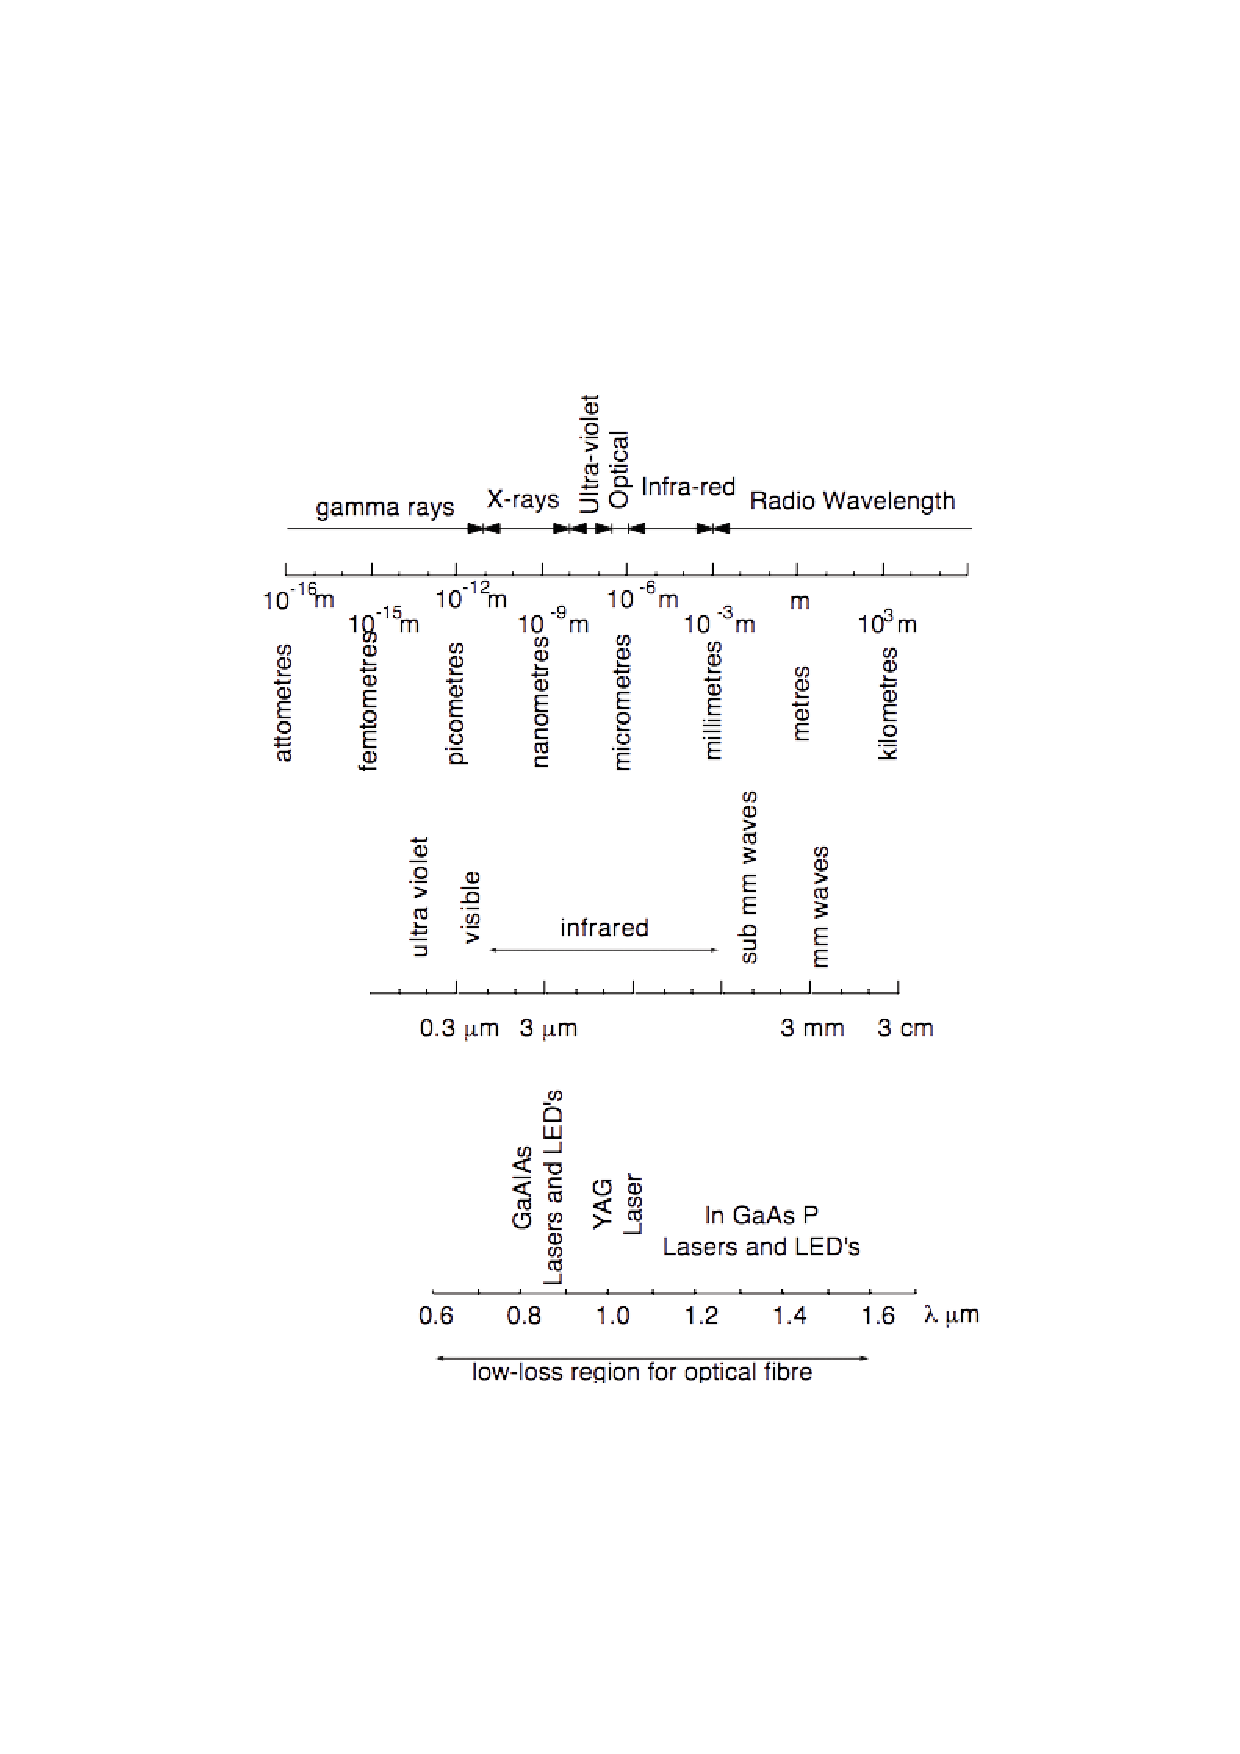
\includegraphics[width=0.75\textwidth]{EMspectrum}}

\def\atmatt{\centering
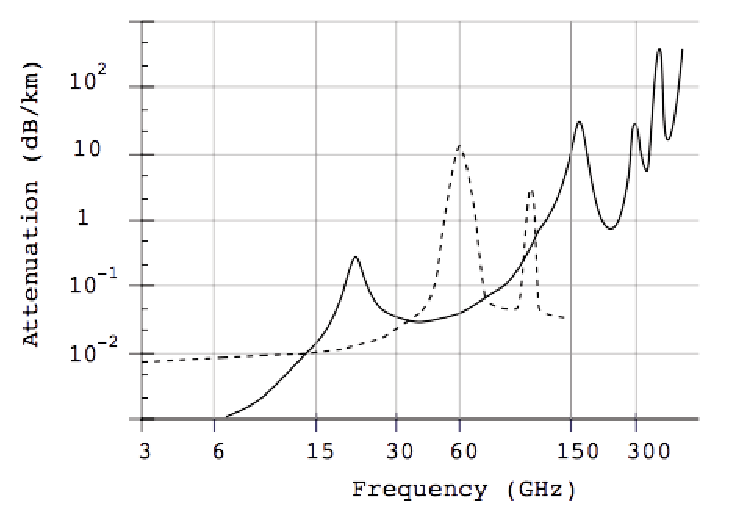
\includegraphics[width=0.75\textwidth]{atmatt3.eps}}


%



%=========================================================================
\section{Coordinate systems}
%=========================================================================


%=========================================================================
\begin{frame}[shrink=20]{Coordinate systems}
%


\begin{figure}
\centering

%Angle Definitions
%-----------------

%set the plot display orientation
%synatax: \tdplotsetdisplay{\theta_d}{\phi_d}
%\tdplotsetmaincoords{60}{110}
\tdplotsetmaincoords{60}{120}

%define polar coordinates for some vector
%TODO: look into using 3d spherical coordinate system
\pgfmathsetmacro{\rvec}{.8}
\pgfmathsetmacro{\thetavec}{30}
\pgfmathsetmacro{\phivec}{60}

%start tikz picture, and use the tdplot_main_coords style to implement the display 
%coordinate transformation provided by 3dplot
\begin{tikzpicture}[scale=5,tdplot_main_coords]

%set up some coordinates 
%-----------------------
\coordinate (O) at (0,0,0);

%determine a coordinate (P) using (r,\theta,\phi) coordinates.  This command
%also determines (Pxy), (Pxz), and (Pyz): the xy-, xz-, and yz-projections
%of the point (P).
%syntax: \tdplotsetcoord{Coordinate name without parentheses}{r}{\theta}{\phi}
\tdplotsetcoord{P}{\rvec}{\thetavec}{\phivec} 

\draw (0.5,0.5,0.5) node[anchor=south]{$z$};
\draw (0.3,0.3,0.0) node[anchor=south]{$\rho$};
\draw (0.25,0.25,0.3) node[anchor=south]{$r$};

%draw figure contents
%--------------------

%draw the main coordinate system axes
\draw[thick,->] (0,0,0) -- (1,0,0) node[anchor=north east]{$X$};
\draw[thick,->] (0,0,0) -- (0,1,0) node[anchor=north west]{$Y$};
\draw[thick,->] (0,0,0) -- (0,0,1) node[anchor=south]{$Z$};

%\draw[thin,->] (0,0,0) -- (0.25,0,0) node[anchor=south]{$x$};


%draw a vector from origin to point (P) 
\draw[-stealth,color=black] (O) -- (P);

%draw projection on xy plane, and a connecting line
\draw[dashed, color=black] (O) -- (Pxy);
\draw[dashed, color=black] (P) -- (Pxy);

%draw the angle \phi, and label it
%syntax: \tdplotdrawarc[coordinate frame, draw options]{center point}{r}{angle}{label options}{label}
\tdplotdrawarc{(O)}{0.2}{0}{\phivec}{anchor=north}{$\phi$}


%set the rotated coordinate system so the x'-y' plane lies within the
%"theta plane" of the main coordinate system
%syntax: \tdplotsetthetaplanecoords{\phi}
\tdplotsetthetaplanecoords{\phivec}

%draw theta arc and label, using rotated coordinate system
\tdplotdrawarc[tdplot_rotated_coords]{(0,0,0)}{0.5}{0}{\thetavec}{anchor=south west}{$\theta$}

%draw some dashed arcs, demonstrating direct arc drawing
\draw[dashed,tdplot_rotated_coords] (\rvec,0,0) arc (0:90:\rvec);
\draw[dashed] (\rvec,0,0) arc (0:90:\rvec);

%%set the rotated coordinate definition within display using a translation
%%coordinate and Euler angles in the "z(\alpha)y(\beta)z(\gamma)" euler rotation convention
%%syntax: \tdplotsetrotatedcoords{\alpha}{\beta}{\gamma}
%\tdplotsetrotatedcoords{\phivec}{\thetavec}{0}
%
%%translate the rotated coordinate system
%%syntax: \tdplotsetrotatedcoordsorigin{point}
%\tdplotsetrotatedcoordsorigin{(P)}
%
%%use the tdplot_rotated_coords style to work in the rotated, translated coordinate frame
%\draw[thick,tdplot_rotated_coords,->] (0,0,0) -- (.5,0,0) node[anchor=north west]{$x'$};
%\draw[thick,tdplot_rotated_coords,->] (0,0,0) -- (0,.5,0) node[anchor=west]{$y'$};
%\draw[thick,tdplot_rotated_coords,->] (0,0,0) -- (0,0,.5) node[anchor=south]{$z'$};
%
%%WARNING:  coordinates defined by the \coordinate command (eg. (O), (P), etc.)
%%cannot be used in rotated coordinate frames.  Use only literal coordinates.  
%
%%draw some vector, and its projection, in the rotated coordinate frame
%\draw[-stealth,color=blue,tdplot_rotated_coords] (0,0,0) -- (.2,.2,.2);
%\draw[dashed,color=blue,tdplot_rotated_coords] (0,0,0) -- (.2,.2,0);
%\draw[dashed,color=blue,tdplot_rotated_coords] (.2,.2,0) -- (.2,.2,.2);
%
%%show its phi arc and label
%\tdplotdrawarc[tdplot_rotated_coords,color=blue]{(0,0,0)}{0.2}{0}{45}{anchor=north west,color=black}{$\phi'$}
%
%%change the rotated coordinate frame so that it lies in its theta plane.
%%Note that this overwrites the original rotated coordinate frame
%%syntax: \tdplotsetrotatedthetaplanecoords{\phi'}
%\tdplotsetrotatedthetaplanecoords{45}
%
%%draw theta arc and label
%\tdplotdrawarc[tdplot_rotated_coords,color=blue]{(0,0,0)}{0.2}{0}{55}{anchor=south west,color=black}{$\theta'$}

\end{tikzpicture}


%\includegraphics{figura.eps}
\caption{Convention for coordinate orientation.}\label{fig:1coord}
\end{figure}

We will use cartesian, circular cylindrical and spherical coordinates systems.

\end{frame}

\section{Coordinates transformations}
\begin{frame}[shrink=00]{Cylindrical Coordinates}
When passing from rectangular to cylindrical coordinates the following transformations apply:
%
\bea
\rho & = & \sqrt{x^2 + y^2} = r \,\sin \theta \nonumber \\
\phi & = & \tan^{-1} \left(\frac{y}{x}\right) \nonumber \\
z & = & r \, \cos \theta
\label{rect2cyl}
\eea
%
\pause
From cylindrical to rectangular:
%
\bea
x & = & \rho \cos \phi \nonumber \\
y & = & \rho \sin \phi  \nonumber \\
z & = & z
\label{cyl2rect}
\eea
%
\pause
The volume element is

\be
dV = \rho \, d\rho \, d\phi \, dz
\ee
\end{frame}

\begin{frame}[shrink=00]{Spherical Coordinates}
Rectangular to spherical
%
\bea
r & = & \sqrt{x^2 + y^2+z^2} = \sqrt{\rho^2 + z^2} \nonumber \\
\theta & = & \tan^{-1} \left(\frac{ \sqrt{x^2 + y^2}}{z}\right) = \tan^{-1} \left(\frac{\rho}{z}\right)\nonumber \\
\phi & = & \tan^{-1} \left(\frac{y}{x}\right) \, .
\label{rect2sph}
\eea
%
\pause
and for the spherical to rectangular
%
\bea
x & = & r \, \sin \theta \, \cos \phi \nonumber \\
y & = & r \, \sin \theta \,\sin \phi  \nonumber \\
z & = & r \cos \theta \, .
\label{sph2rect}
\eea
%
\pause
The volume element is

\be
dV = r^2 \sin \theta \, dr  \, d\theta \, d\phi 
\ee

\end{frame}

\begin{frame}[shrink=00]{Examples}
Before proceeding further complete examples 3.4, 3.5, 3.6
\end{frame}

\section{Unit vectors}
%
\begin{frame}[shrink=00]{Unit vectors: transformations from cylindrical/spherical to rectangular}
\alert{The coordinate unit vectors are defined as vectors of unit length pointing along coordinate lines in the direction of increasing coordinate variables.}
\pause

It is left as an exercise to draw them in the three coordinate systems. 
\pause
The following rules are applicable to transformations among unit coordinate vectors.

Transformations from cylindrical/spherical to rectangular:
%
\bea
\Bu_x & = & \Bu_\rho \, \cos \phi - \Bu_\phi \, \sin \phi \nonumber \\
& = & \Bu_r \, \sin \theta \, \cos \phi  + \Bu_\theta \, \cos \theta \, \cos \phi- \Bu_\phi \, \sin \phi  \nonumber \\
\Bu_y & = & \Bu_\rho \, \sin \phi + \Bu_\phi \, \cos \phi \nonumber \\
& = & \Bu_r \, \sin \theta \, \sin \phi  + \Bu_\theta \, \cos \theta \, \sin \phi + \Bu_\phi \, \cos \phi  \nonumber \\
\Bu_z & = & \Bu_r \, \cos \theta -  \Bu_\theta \, \sin \theta
\label{cylsph2rectu}
\eea
%
\pause
\end{frame}
%
\begin{frame}[shrink=00]{Transformations from rectangular/spherical to cylindrical}

Transformations from rectangular/spherical to cylindrical

%
\bea
\Bu_\rho & = & \Bu_x \, \cos \phi + \Bu_y \, \sin \phi \nonumber 
%\\& = & 
= \Bu_r \, \sin \theta   + \Bu_\theta \, \cos \theta  \nonumber \\
\Bu_\phi & = & - \Bu_x \, \sin \phi + \Bu_y \, \cos \phi \nonumber \\
\Bu_z & = & \Bu_r \, \cos \theta -  \Bu_\theta \, \sin \theta
\label{rectsph2cylu}
\eea
%

\end{frame}
%
\begin{frame}[shrink=00]{Transformations from rectangular/cylindrical to spherical}

Transformations from rectangular/cylindrical to spherical:
%
\bea
\Bu_r & = & \Bu_x \, \sin \theta \, \cos \phi + \Bu_y \, \sin \theta \, \sin \phi + \Bu_z \, \cos \theta \nonumber \\
& = & \Bu_\rho \, \sin \theta  + \Bu_z \, \cos \theta   \nonumber \\
\Bu_\theta & = & \Bu_x \, \cos \theta \, \cos \phi + \Bu_y \,  \cos \theta \, \sin \phi - \Bu_z \, \sin \theta \nonumber \\
& = & \Bu_\rho \, \cos \theta  - \Bu_z \, \sin \theta  \nonumber \\
\Bu_\phi & = & - \Bu_x \, \sin \phi +  \Bu_y \, \cos \phi
\label{rectcyl2sphu}
\eea
%
\end{frame}

\section{Coordinate transformations for vector components}
%
\begin{frame}[shrink=00]{Coordinate transformations for vector components}

%\begin{enumerate}[label={\alph*)}]
%\item 
Rectangular to cylindrical components
\bea
F_\rho  & = & F_x \, \cos \phi + F_y \, \sin \phi \nonumber \\
F_\phi & = & - F_x \, \sin \phi +  F_y \, \cos \phi \nonumber \\
F_z & = & F_z
\eea
%
%\item
 \pause
 
Rectangular to spherical components
\bea
F_r  & = & F_x \, \sin \theta \, \cos \phi + F_y \, \sin \theta \, \sin \phi  + F_z \cos \theta\nonumber \\
F_\theta & = &  F_x \, \cos \theta \, \cos \phi +  F_y \, \cos \theta \, \sin \phi  - F_z \sin \theta\nonumber \\
F_\phi & = &  - F_x \, \sin \phi +  F_y \, \cos \phi
\eea
%
\end{frame}
%


\begin{frame}[shrink=00]{}

%\item 
Cylindrical to rectangular components
\bea
F_x  & = & F_\rho \,  \cos \phi - F_\phi \, \sin \phi  \nonumber \\
F_y & = &  F_\rho \,  \sin \phi +  F_\phi \,  \cos \phi \ \nonumber \\
F_z & = &  F_z
\eea
%
%\item 

\pause
Cylindrical to spherical components
\bea
F_r  & = & F_\rho \, \sin \theta + F_z \, \cos \theta \nonumber \\
F_\theta & = & F_\rho \, \cos \theta -  F_z \, \sin \theta \nonumber \\
F_\phi & = & F_\phi
\eea
%

\end{frame}


%
\begin{frame}[shrink=00]{Coordinate systems}
 
%\item 
Spherical to rectangular components
\bea
F_x  & = & F_r \, \sin \theta \, \cos \phi + F_\theta \, \cos \theta \, \cos \phi  - F_\phi \, \sin \phi\nonumber \\
F_y & = &  F_r \, \sin \theta \, \sin \phi +  F_\theta \, \cos \theta \, \sin \phi  + F_\phi \cos \phi \nonumber \\
F_z & = &   F_r \, \cos \theta -  F_\theta \, \sin \phi
\eea
%

\pause
%\item 
Spherical to cylindrical components
\bea
F_\rho  & = & F_r \,  \sin \theta +  F_\theta \, \cos \theta  \nonumber \\
F_\phi & = &  F_\phi \nonumber \\
F_z & = &  F_r \,  \cos \theta -  F_\theta \, \sin \theta 
\eea
%
%\end{enumerate}

\end{frame}

\begin{frame}[shrink=00]{Summary of coordinate transformations:r2c}

\newpage
\small
\lstinputlisting{wxMaxima/coordinate_transf/r2c.wxm}
\normalsize
\newpage
\end{frame}

\begin{frame}[shrink=00]{Summary of coordinate transformations:c2r}

\newpage
\small
\lstinputlisting{wxMaxima/coordinate_transf/c2r.wxm}
\normalsize
\newpage
\end{frame}

\begin{frame}[shrink=00]{Summary of coordinate transformations: r2s}

\newpage
\small
\lstinputlisting{wxMaxima/coordinate_transf/r2s.wxm}
\normalsize
\newpage
\end{frame}

\begin{frame}[shrink=00]{Summary of coordinate transformations: s2r}

\newpage
\small
\lstinputlisting{wxMaxima/coordinate_transf/s2r.wxm}
\normalsize
\newpage
\end{frame}

\begin{frame}[shrink=00]{Summary of coordinate transformations: c2s}

\newpage
\small
\lstinputlisting{wxMaxima/coordinate_transf/c2s.wxm}
\normalsize
\newpage
\end{frame}

\begin{frame}[shrink=00]{Summary of coordinate transformations: s2c}

\newpage
\small
\lstinputlisting{wxMaxima/coordinate_transf/s2c.wxm}
\normalsize
\newpage
\end{frame}

%__________________________________________________________
\begin{frame}[shrink=00]{Summary of vector transformations: v r2c}

\newpage
\small
\lstinputlisting{wxMaxima/vector_transf/v_r2c.wxm}
\normalsize
\newpage
\end{frame}


%__________________________________________________________
\begin{frame}[shrink=00]{Summary of vector transformations: v c2r}

\newpage
\small
\lstinputlisting{wxMaxima/vector_transf/v_c2r.wxm}
\normalsize
\newpage
\end{frame}


%__________________________________________________________
\begin{frame}[shrink=00]{Summary of vector transformations: v r2s}

\newpage
\small
\lstinputlisting{wxMaxima/vector_transf/v_r2s.wxm}
\normalsize
\newpage
\end{frame}


%__________________________________________________________
\begin{frame}[shrink=00]{Summary of vector transformations: v s2r}

\newpage
\small
\lstinputlisting{wxMaxima/vector_transf/v_s2r.wxm}
\normalsize
\newpage
\end{frame}


%__________________________________________________________
\begin{frame}[shrink=00]{Summary of vector transformations: v c2s}

\newpage
\small
\lstinputlisting{wxMaxima/vector_transf/v_c2s.wxm}
\normalsize
\newpage
\end{frame}


%__________________________________________________________
\begin{frame}[shrink=00]{Summary of vector transformations: v s2c}

\newpage
\small
\lstinputlisting{wxMaxima/vector_transf/v_s2c.wxm}
\normalsize
\newpage
\end{frame}



\section{Pauli matrices in Cylindrical coordinates}

%\subsubsection{Pauli matrices for the cylindrical coordinate system}



\begin{frame}[shrink=00]{Pauli matrices in Cylindrical coordinates}

We have already introduced the Pauli matrices for the rectangular coordinate system $\sigma_i$, with $i=0,\ldots,3$.
When expressing a vector can identify $\sigma_1$ with $\Bu_x$, $\sigma_2$ with $\Bu_y$ and $\sigma_3$ with $\Bu_z$.
By using (\ref{rectsph2cylu}) we can write:
\bea
\Bu_\rho & = & \Bu_x \, \cos \phi + \Bu_y \, \sin \phi \nonumber \\
\sigma_\rho & = & \cos \phi \sigma_1 + \sin \phi \sigma_2 \nonumber \\
& = & \begin{pmatrix}0 & {e}^{-i\,\phi}\cr {e}^{i\,\phi} & 0\end{pmatrix} \, .
\eea
\pause
Similarly, for the unit vector along $\phi$ we can write
\bea
\Bu_\phi & = & - \Bu_x \, \sin \phi + \Bu_y \, \cos \phi \nonumber \\
\sigma_\phi & = & - \sin \phi \sigma_1 + \cos \phi \sigma_2 \nonumber \\
& = & \begin{pmatrix}0 & -i\,{e}^{-i\,\phi}\cr i\,{e}^{i\,\phi} & 0\end{pmatrix} \, .
\eea
%
\end{frame}


\begin{frame}[shrink=00]{Pauli matrices in Cylindrical coordinates}
Naturally, for the $z$ component we have that $\sigma_z=\sigma_3$.
Summarizing, we have the following three matrices in cylindrical coordinates


\bea
\sigma_\rho & = &  \begin{pmatrix}0 & {e}^{-i\,\phi}\cr {e}^{i\,\phi} & 0\end{pmatrix} \nonumber \\
\sigma_\phi & = & \begin{pmatrix}0 & -i\,{e}^{-i\,\phi}\cr i\,{e}^{i\,\phi} & 0\end{pmatrix} \nonumber \\
\sigma_z & = & \begin{pmatrix}1 & 0\cr 0 & -1\end{pmatrix} \, .
\label{sigma_cyl}
\eea

\end{frame}

\begin{frame}{Pauli matrices in Cylindrical coordinates}
It is readily proved that the matrices $\sigma_\rho, \sigma_\phi, \sigma_z$ when multiplied by themselves give the identity matrix $\sigma_0$, their trace is null, their determinant is always $-1$ and their dot product is zero if they are not the same. 
\pause
In addition we have
\bea
i \, \sigma_z & = & \sigma_\rho \sigma_\phi \nonumber \\
i \, \sigma_\rho & = & \sigma_\phi \sigma_z \nonumber \\
i \, \sigma_\phi & = & \sigma_z \sigma_\rho \, .
\eea
\pause
Therefore the generic vector $\BA$ can be expressed in cylindrical coordinates in terms of Pauli matrices as
\bea
\tilde{A} & =  & A_\rho \sigma_\rho + A_\phi \sigma_\phi + A_z \sigma_z \nonumber \\
& = & \begin{pmatrix}{A}_{z} & {e}^{-i\,\phi}\,\left( {A}_{\rho}-i\,{A}_{\phi}\right) \cr {e}^{i\,\phi}\,\left( {A}_{\rho} + i\,{A}_{\phi}\right)  & -{A}_{z}\end{pmatrix} \,.
\label{rectcyl}
\eea
%It is noted that since the vector is the same when expressed in rectangular or cylindrical components we have the identity
%\be
%A_\rho \sigma_\rho + A_\phi \sigma_\phi + A_z \sigma_z=
%A_x \sigma_1 + A_y \sigma_2 + A_z \sigma_3 \, .
%\ee
\end{frame}


\begin{frame}[shrink=00]{Pauli matrices in Cylindrical coordinates}
It is noted that since the vector is the same when expressed in rectangular or cylindrical components we have the identity
\be
A_\rho \sigma_\rho + A_\phi \sigma_\phi + A_z \sigma_z=
A_x \sigma_1 + A_y \sigma_2 + A_z \sigma_3 \, .
\ee

By performing the dot product of the above expression with a selected sigma matrix we can recover the desired field component in terms of the other basis.

\end{frame}


\begin{frame}[shrink=00]{Pauli matrices in Cylindrical coordinates}

As an example let us consider to retrieve the expression of $A_\rho$ in terms of the rectangular components. 
\pause
It is sufficient to dot multiply both sides of (\ref{rectcyl}) times $\sigma_\rho$ to retrieve
\bea 
A_\rho & =  & A_x \sigma_1 \cdot \sigma_\rho + A_y \sigma_2 \cdot \sigma_\rho + A_z \sigma_3 \cdot \sigma_\rho \nonumber \\
& =  & {{A}_{x} \, \cos \phi + A}_{y}\,  \sin \phi 
\eea
where we remind that performing  the dot product is equivalent to perform the matrix product and take half of the trace.
It is left as an exercise for the reader to recover the results in the previous section by using Pauli matrices multiplication.


\end{frame}

\begin{frame}[shrink=80]{Pauli matrices in Cylindrical coordinates}


\newpage
\small
\lstinputlisting{Pauli_cyl_v2.wxm}
\normalsize
\newpage

\end{frame}


%%%%%%%%%%%%%%%%%%%%%%%%%%%%%%%%%%%%%%%%%%%%%%%%
\section{Pauli matrices in Spherical coordinates}
%%%%%%%%%%%%%%%%%%%%%%%%%%%%%%%%%%%%%%%%%%%%%%%%
%\subsection{Pauli matrices for the spherical coordinate system}






 
 
\begin{frame}[shrink=00]{Pauli matrices in Spherical coordinates}
So far we have introduced the Pauli matrices for the rectangular and cylindrical coordinate systems. We can proceed in the same way that we have followed for the cylindrical coordinate system.
\pause
By using (\ref{rectcyl2sphu}) we can write:
\bea
\Bu_r & = & \Bu_x \, \sin \theta \, \cos \phi + \Bu_y \, \sin \theta \, \sin \phi + \Bu_z \, \cos \theta \nonumber \\
\sigma_r & = &  \sin \theta \, \cos \phi \, \sigma_1+  \sin \theta \, \sin \phi \, \sigma_2 +  \cos \theta \, \sigma_3 \nonumber \\
& = & \begin{pmatrix}\cos \theta  & {e}^{-i\,\phi}\, \sin \theta \cr {e}^{i\,\phi}  \, \sin \theta & -\cos \theta \end{pmatrix} \, .
\eea

\end{frame}

\begin{frame}[shrink=00]{Pauli matrices in Spherical coordinates}

Similarly, for the unit vector along $\theta$ we can write:

\bea
\Bu_\theta & = & \Bu_x \, \cos \theta \, \cos \phi + \Bu_y \,  \cos \theta \, \sin \phi - \Bu_z \, \sin \theta \nonumber \\
\sigma_\theta & = &  \cos \theta \, \cos \phi  \, \sigma_1+  \cos \theta \, \sin \phi \, \sigma_2 - \sin \theta \, \sigma_3 \nonumber \\
& = & \begin{pmatrix}-\sin\theta & {e}^{-i\,\phi}\, \cos \theta \cr {e}^{i\,\phi}  \, \cos \theta& \sin \theta \end{pmatrix} \, .
\eea
%
\pause
Not surprisingly for the $\phi$ coordinate the result is the same as in cylindrical coordinates.
\end{frame}
%


\begin{frame}[shrink=0]{Pauli matrices in Spherical coordinates}

Summarizing, we have the following three matrices in spherical coordinates
\bea
\sigma_r & = &  \begin{pmatrix}\cos \theta  & {e}^{-i\,\phi}\, \sin \theta \cr {e}^{i\,\phi}  \, \sin \theta & -\cos \theta \end{pmatrix} \nonumber \\
\sigma_\theta & = &  \begin{pmatrix}-\sin\theta & {e}^{-i\,\phi}\, \cos \theta \cr {e}^{i\,\phi}  \, \cos \theta& \sin \theta \end{pmatrix} \nonumber \\
\sigma_\phi & = & \begin{pmatrix}0 & -i\,{e}^{-i\,\phi}\cr i\,{e}^{i\,\phi} & 0\end{pmatrix} \, .
\label{sigma_sph}
\eea
\end{frame}

\begin{frame}[shrink=0]{Pauli matrices in Spherical coordinates}

It is readily proved that the matrices $\sigma_r, \sigma_\theta, \sigma_\phi$ when multiplied by themselves give the identity matrix $\sigma_0$, their trace is null, their determinant is always $-1$ and their dot product is zero if they are not the same. In addition we have:

\bea
i \, \sigma_\phi & = & \sigma_r \sigma_\theta \nonumber \\
i \, \sigma_r & = & \sigma_\theta \sigma_\phi \nonumber \\
i \, \sigma_\theta & = & \sigma_\phi \sigma_r \, .
\eea
\end{frame}

\begin{frame}[shrink=20]{Pauli matrices in Spherical coordinates}
Therefore, the generic vector $\BA$ can be expressed in spherical coordinates in terms of Pauli matrices as:

\bea
\tilde{A} & =  & A_r \sigma_r + A_\theta \sigma_\theta + A_\phi \sigma_\phi \nonumber \\
& = & 
\begin{pmatrix} {A}_{r}\, \cos \theta-{A}_{\theta}\,\sin \theta  & 
{e}^{-i\,\phi}\,\left({A}_{r}\, \sin \theta \,-i \,{A}_{\phi}+{A}_{\theta}\,\cos \theta\right) \cr 
{e}^{i\,\phi}\,\left({A}_{r}\, \sin \theta \,+i \,{A}_{\phi}+{A}_{\theta}\,\cos \theta\right) & 
-{A}_{r}\, \cos \theta+{A}_{\theta}\,\sin \theta
\end{pmatrix} 
\label{rectcyl}
\eea

\end{frame}

\begin{frame}[shrink=00]{Pauli matrices in Spherical coordinates}

It is noted that since the vector is the same when expressed in rectangular, cylindrical or spherical components we have the identity
\bea
\tilde{A} & = & A_x \sigma_1 + A_y \sigma_2 + A_z \sigma_3 \nonumber \\
& = & A_\rho \sigma_\rho + A_\phi \sigma_\phi + A_z \sigma_z \nonumber \\
& = &A_r \sigma_r + A_\theta \sigma_\theta + A_\phi \sigma_\phi \, .
\eea
\pause
By performing the dot product of the above expression with a selected sigma matrix we can recover the desired field component in terms of the other basis.

Thus all the transformation between vectors in different coordinate systems can be simply obtained by matrix multiplication and trace operation.

\end{frame}

\begin{frame}[shrink=00]{Pauli matrices in Spherical coordinates}

\newpage
\small
\lstinputlisting{Pauli_sph_1.wxm}
\normalsize
\newpage
\end{frame}

\begin{frame}[shrink=00]{Pauli matrices in Spherical coordinates}
An example of application is provided with the following listing.
% \newpage
\small
\lstinputlisting{example_Pauli_sph.wxm}
\normalsize
\newpage
\end{frame}


%\begin{frame}[shrink=20]{Coordinate systems}
%\end{frame}
%
%\begin{frame}[shrink=20]{Coordinate systems}
%\end{frame}
%
%\begin{frame}[shrink=20]{Coordinate systems}
%\end{frame}
%
%\begin{frame}[shrink=20]{Coordinate systems}
%\end{frame}

%\begin{frame}[shrink=20]{Coordinate systems}
%\end{frame}
%\begin{frame}[shrink=20]{Coordinate systems}
%\end{frame}
%
%\begin{frame}[shrink=20]{Coordinate systems}
%\end{frame}
%
%\begin{frame}[shrink=20]{Coordinate systems}
%\end{frame}
%
%\begin{frame}[shrink=20]{Coordinate systems}
%\end{frame}
%
%\begin{frame}[shrink=20]{Coordinate systems}
%\end{frame}
%
%\begin{frame}[shrink=20]{Coordinate systems}
%\end{frame}
%
%\begin{frame}[shrink=20]{Coordinate systems}
%\end{frame}
%
%\begin{frame}[shrink=20]{Coordinate systems}
%\end{frame}
%
%\begin{frame}[shrink=20]{Coordinate systems}
%\end{frame}
%
%\begin{frame}[shrink=20]{Coordinate systems}
%\end{frame}
%
%\begin{frame}[shrink=20]{Coordinate systems}
%\end{frame}



\end{document}
